\textbf{3-1.} 一横截面积为 $S = 20\mathrm{cm}^2$ 的空心螺绕环，每厘米长度上绕有50匝，环外绕有5匝的副线圈，副线圈与电流计串联，构成一个电阻为 $R = 2.0\Omega$ 的闭合回路。今使螺绕环中的电流每秒减少 $20\mathrm{A}$ ，求副线圈中的感应电动势 $\mathcal{E}$ 和感应电流。

\vfill

\textbf{3-2.} 一正方形线圈每边长 $100\mathrm{mm}$ , 在地磁场中转动, 每秒转 30 圈; 转轴通过中心并与一边平行, 且与地磁场 $\pmb{B}$ 垂直。

(1) 线圈法线与地磁场 $B$ 的夹角为什么值时，线圈中产生的感应电动势最大？

(2) 设地磁场的$B=0.55Gs$，这时要在线圈中最大产生$10mV$的感应电动势，求线圈的匝数$N$.

\vfill
\newpage

\textbf{3-3.} 如本题图所示, 一很长的直导线有交变电流 $i(t) = I_0 \sin \omega t$ , 它旁边有一长方形线圈 $ABCD$ , 长为 $l$ , 宽为 $(b - a)$ , 线圈和导线在同一平面内。求:

(1) 穿过回路 $ABCD$ 的磁通量 $\Phi$ ;

(2) 回路 $ABCD$ 中的感应电动势 $\mathcal{E}$.


\vfill

\textbf{3-4.} 一长直导线载有5.0A的直流电流，旁边有一个与它共面的矩形线圈, 长 $l=20\ cm$ , $a=10\ cm$ , $b=20\ cm$ , 如本题图所示; 线圈共有 N=1000 匝, 以 v=3.0m/s 的速度离开直导线。求图示位置的感应电动势的大小和方向。

\vfill
\newpage

\textbf{3-5.} 如本题图, 电流为 $I$ 的长直导线附近有正方形线圈绕中心轴 $OO'$ 以匀角速度 $\omega$ 旋转, 求线圈中的感应电动势。已知正方形边长为 $2a$ , $OO'$ 轴与长导线平行, 相距为 $b$ .

\begin{center}
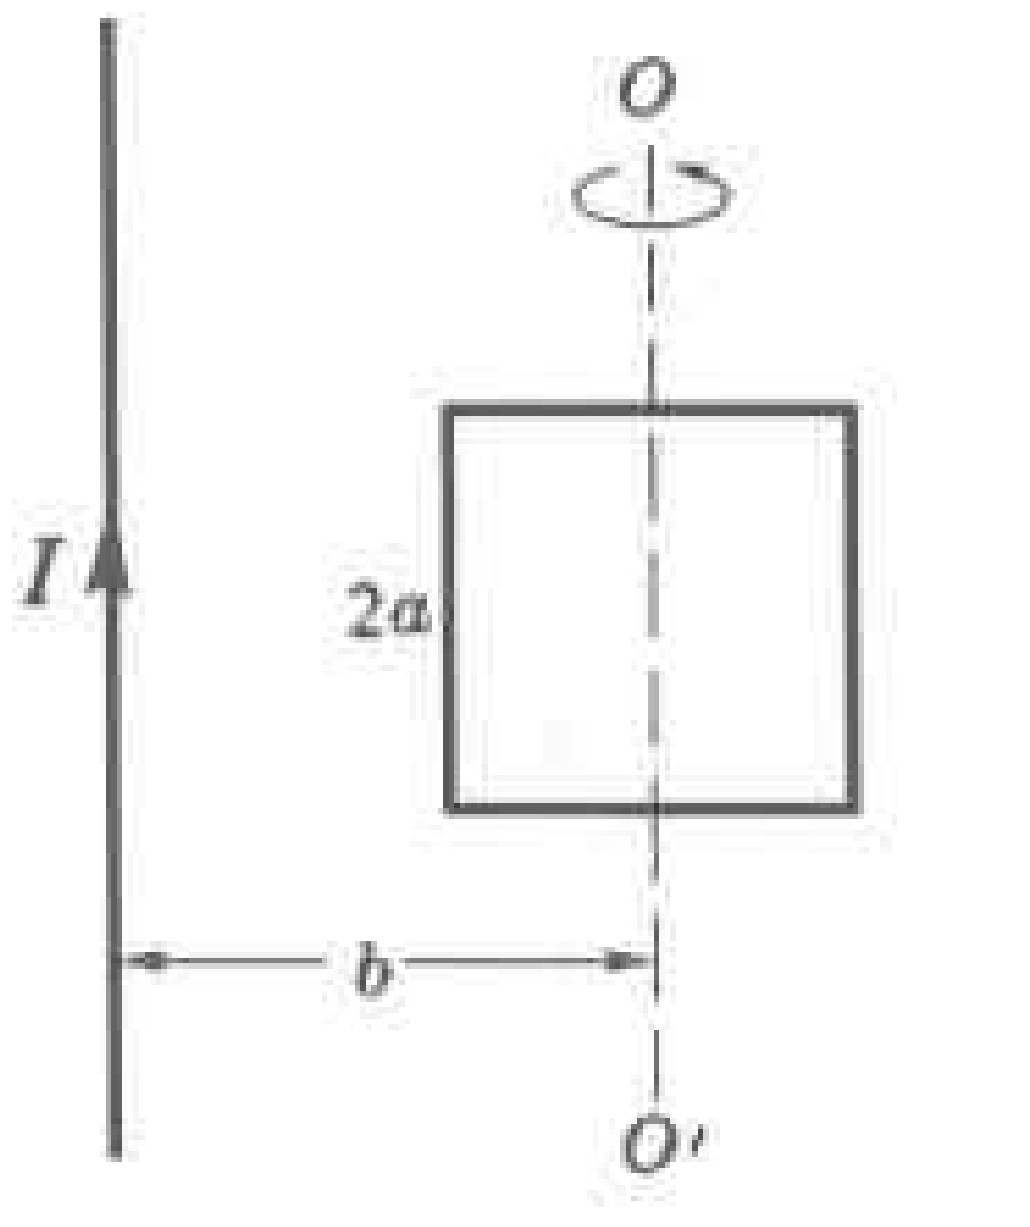
\includegraphics[width=0.2\linewidth]{figures/习题3-5.jpg}
\end{center}

\vfill

\textbf{3-6.} 本题图中导体棒 $AB$ 与金属轨道 $CA$ 和 $DB$ 接触，整个线框放在 $B = 0.50\mathrm{T}$ 的均匀磁场中，磁场方向与图画垂直。
\begin{center}
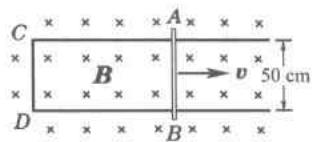
\includegraphics[width=0.3\linewidth]{figures/习题3-6.jpg}
\end{center}
(1)若导体棒以 $4.0 m/s$ 的速度向右运动，求棒内感应电动势的大小和方向；

(2) 若导体棒运动到某一位置时, 电路的电阻为 $0.20 \Omega$ , 求此时棒所受的力。摩擦力可不计。

(3) 比较外力作功的功率和电路中所消耗的热功率。

\vfill
\newpage

\textbf{3-7.} 闭合线圈共有 $N$ 匝, 电阻为 $R$ . 证明: 当通过这线圈的磁通量改变 $\Delta \Phi$ 时, 线圈内流过的电荷量为
$$
\Delta q = \frac {N \Delta \Phi}{R}.
$$

\vfill

\textbf{3-8.} 本题图所示为测量螺线管中磁场的一种装置。把一个很小的测量线圈放在待测处，这线圈与测量电荷量的冲击电流计G串联。冲击电流计是一种可测量迁移过它的电荷量的仪器。当用反向开关K使螺线管的电流反向时，测量线圈中就产生感应电动势，从而产生电荷量 $\Delta q$ 的迁移；由G测出 $\Delta q$ 就可以算出测量线圈所在处的 $B$ .已知测量线圈有2000匝，它的直径为2.5cm，它和G串联回路的电阻为1000Ω，在K反向时测得 $\Delta q=2.5\times10^{-7}C$ 。求被测处的磁感应强度。
\begin{center}
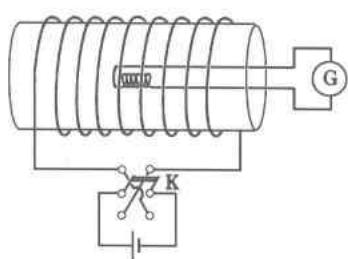
\includegraphics[width=0.3\linewidth]{figures/习题3-8.jpg}
\end{center}


\vfill
\newpage

\textbf{3-9.} 如本题图所示, 线圈 $abcd$ 放在 $B = 6.0 \times 10^{3} \mathrm{Gs}$ 的均匀磁场中, 磁场方向与线圈平面法线的夹角 $\alpha = 60^{\circ}$ , $ab$ 长 $1.0 \mathrm{~m}$ , 可左右运动。今使 $ab$ 以 $v = 5.0 \mathrm{~m} / \mathrm{s}$ 的速度向右运动, 求感应电动势的大小及感应电流的方向。
\begin{center}
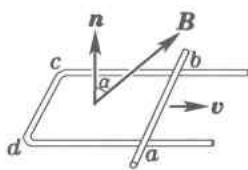
\includegraphics[width=0.3\linewidth]{figures/习题3-9.jpg}
\end{center}



\vfill

\textbf{3-10.} 两段导线 $ab = bc = 10\mathrm{cm}$ ，在 $b$ 处相接而成 $30^{\circ}$ 角。若使导线在匀强磁场中以速率 $v = 1.5\mathrm{m / s}$ 运动，方向如本题图所示，磁场方向垂直图面向内， $B = 2.5\times 10^{2}\mathrm{Gs}$ ，问 $ac$ 间的电势差是多少？哪一端的电势高？
\begin{center}
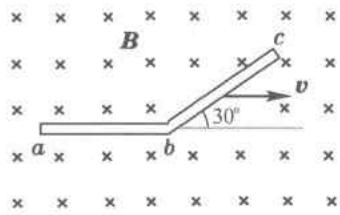
\includegraphics[width=0.3\linewidth]{figures/习题3-10.jpg}
\end{center}

\vfill
\newpage

\textbf{3-11.} 如本题图,金属棒 $ab$ 以 $v = 2.0 \mathrm{~m} / \mathrm{s}$ 的速率平行于一长直导线运动,此导线内有电流 $I = 40 \mathrm{~A}$ . 求棒中感应电动势的大小。哪一端的电势高?
\begin{center}
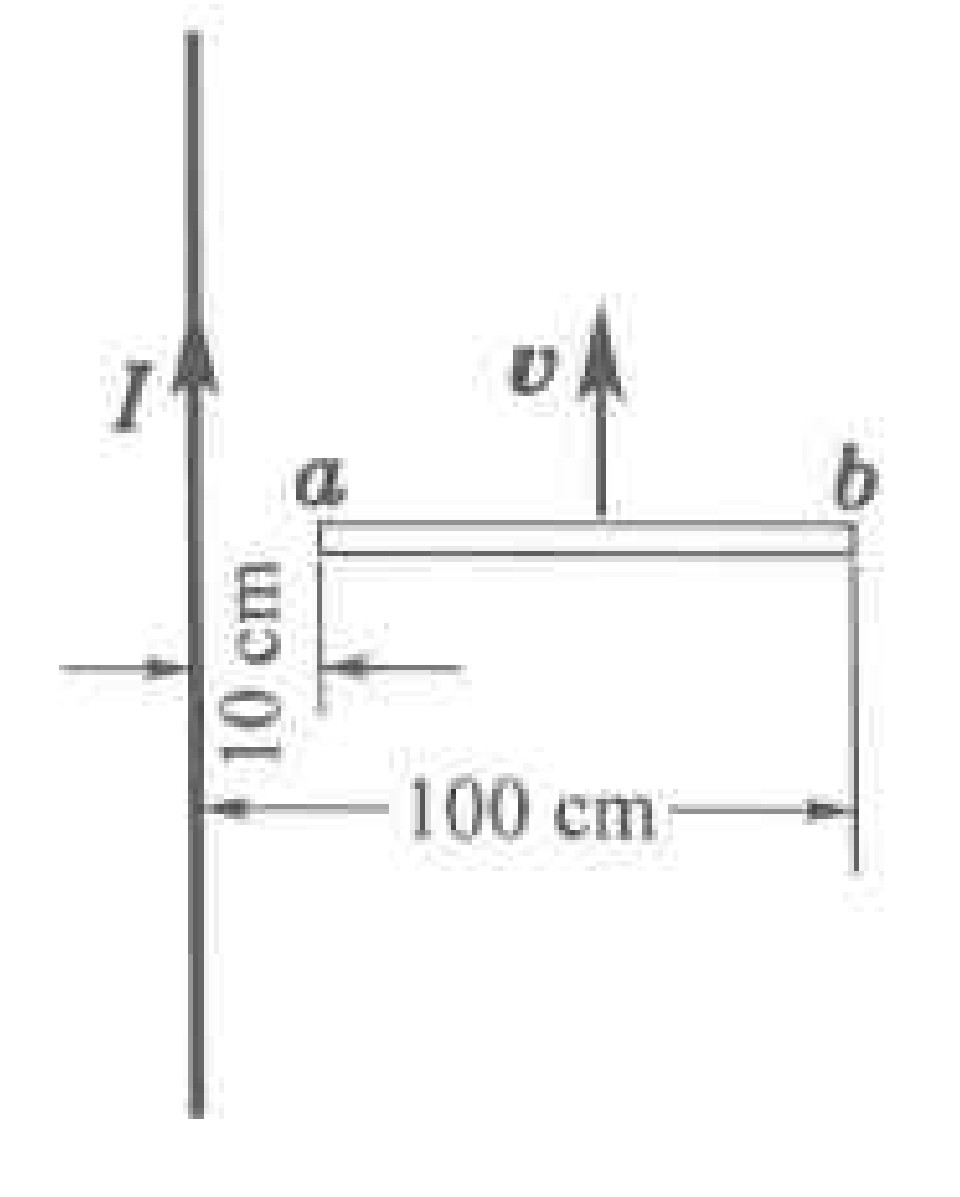
\includegraphics[width=0.25\linewidth]{figures/习题3-11.jpg}
\end{center}


\vfill

\textbf{3-12.} 如本题图，一金属棒长为 $0.50\mathrm{m}$ 水平放置，以长度的1/5处为轴，在水平面内旋转，每秒转两转。已知该处地磁场在竖直方向上的分量 $B_{\perp} = 0.50\mathrm{Gs}$ ，求 $a, b$ 两端的电势差。
\begin{center}
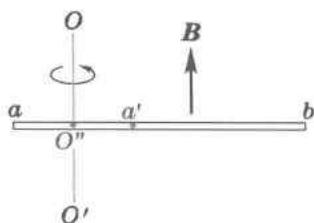
\includegraphics[width=0.3\linewidth]{figures/习题3-12.jpg}
\end{center}

\vfill
\newpage

\textbf{3-13.} 只有一根辐条的轮子在均匀外磁场 $\pmb{B}$ 中转动，轮轴与 $\pmb{B}$ 平行，如本题图所示。轮子和辐条都是导体，辐条长为 $R$ ，轮子每秒转 $N$ 圈。两根导线 $a$ 和 $b$ 通过各自的刷子分别与轮轴和轮边接触。

(1) 求 a、b 间的感应电动势 E；

(2) 若在 a、b 间接一个电阻, 使辐条中的电流为 I, 问 I 的方向如何?

(3) 求这时磁场作用在辐条上的力矩的大小和方向；

(4) 当轮反转时，I 是否也会反向？

(5) 若轮子的辐条是对称的两根或更多根, 结果如何?
\begin{center}
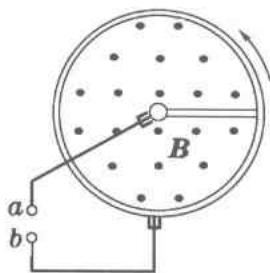
\includegraphics[width=0.25\linewidth]{figures/习题3-13.jpg}
\end{center}

\vfill

\textbf{3-14.} 法拉第圆盘发电机是一个在磁场中转动的导体圆盘。设圆盘的半径为 $R$ ，它的轴线与均匀外磁场 $\pmb{B}$ 平行，它以角速度 $\omega$ 绕轴线转动，如本题图所示。

(1) 求盘边与盘心间的电势差 U;

(2) 当 $R = 15 \, cm, B = 0.60 \, T$ ，转速为每秒 30 圈时，U 等于多少？

(3)盘边与盘心哪处电势高？当盘反转时，它们电势的高低是否也会反过来？
\begin{center}
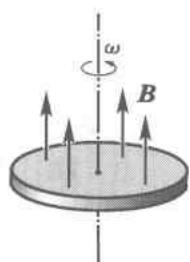
\includegraphics[width=0.2\linewidth]{figures/习题3-14.jpg}
\end{center}

\vfill
\newpage

\textbf{3-15.} 已知在电子感应加速器中, 电子加速的时间是 $4.2 \mathrm{~ms}$ , 电子轨道内最大磁通量为 $1.8 \mathrm{~Wb}$ , 试求电子沿轨道绕行一周平均获得的能量。若电子最终获得的能量为 $100 \mathrm{MeV}$ , 电子绕了多少周? 若轨道半径为 $84 \mathrm{~cm}$ , 电子绕行的路程有多少?

\vfill

\textbf{3-16.} 如本题图所示, 一对同轴圆柱形导体, 半径分别为 $a$ 和 $b$ , 内柱载有沿柱轴 $z$ 方向的电流 $I$ , 电流沿外柱流回。

(1) 求两柱之间区域内的磁矢势表达式；

(2) 一电子从内柱以速率 $v_{0}$ 垂直于柱轴出发, 这电子能达到外柱的最小 $v_{0}$ 值为多少?
\begin{center}
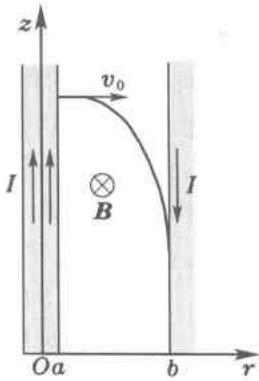
\includegraphics[width=0.2\linewidth]{figures/习题3-16.jpg}
\end{center}

\vfill
\newpage

\textbf{3-17.} 柱形磁控管如本题图所示，设内、外柱半径分别为 $a$ 和 $b$ . 两极间加电压 $U_{0}$ ，处于轴向匀强磁场 $B$ 中。电子以可忽略的初速从阴极 $\mathbf{K}$ 出发，它一方面在径向电场的作用下加速，同时在磁场的作用下偏转，电子将沿心脏线轨迹运动。当磁场超过某临界值 $B_{\mathrm{c}}$ 时，电子不能达到阳极A. 因 $B_{\mathrm{c}}$ 与荷质比 $e / m$ 有关，1921年A.W.Hull首先用此法测量了电子的荷质比。试证明电子的荷质比与临界磁场的关系为：
$$
\frac {e}{m} = \frac {8 U _ {0}}{b ^ {2} B _ {\mathrm{c}} ^ {2}} \frac {1}{\left(1 - \frac {a ^ {2}}{b ^ {2}}\right) ^ {2}}.
$$
\begin{center}
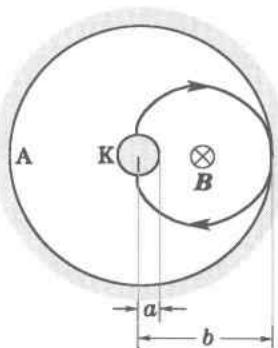
\includegraphics[width=0.2\linewidth]{figures/习题3-17.jpg}
\end{center}


\vfill

\textbf{3-18.} 证明 $E^{2} - c^{2}B^{2}$ 和 $\pmb{B}\cdot \pmb{E}$ 是洛伦兹变换下的不变量。由此可以推论：

(1) 如果在一个参考系中 $E > cB$，则在任意其它参考系中也有 $E > cB$；

(2) 如果在一个参考系中 $E$ 和 $B$ 正交, 则在任意其它参考系中, 它们也正交;

(3)如果在一个参考系中 $E$ 和 $B$ 之间的夹角为锐角（或钝角），则在任意其它参考系中，它们之间的夹角也是锐角（或钝角）。

\vfill
\newpage

\textbf{3-19.} 在某一参考系K中有电场和磁场分别为 $\pmb{E}$ 和 $\pmb{B}$ ，它们满足什么条件时，可以找到另外的参考系 $\mathbf{K}'$ ，使得

（1） $\pmb{E}'$ 和 $\pmb{B}'$ 垂直；

（2） $\pmb{B}' = 0$ ；

（3） $\pmb{E}' = 0$ 。

\vfill

\textbf{3-20.} 已知在 $\mathbf{K}^{\prime}$ 系中一根无限长直带正电的细棒静止，且沿 $x^{\prime}$ 轴放置。其电荷线密度 $\eta_{\mathrm{e}}^{\prime}$ 均匀。设 $\mathbf{K}^{\prime}$ 系相对于 $\mathbf{K}$ 系以速度 $v$ 沿 $x$ 轴正向运动。

(1) 求在 K 系中空间的电场；

(2) 求在 K 系中空间的磁场；

(3)在 K 系中看来，运动的带电细棒相当于无限长直电流，它所产生的磁场服从毕奥-萨伐尔定律，由此证明 $\varepsilon_{0}\mu_{0}=1/c^{2}$ .

\vfill
\newpage

\textbf{3-21.} 在无限大带正电的平面为静止的参考系中，观测到该平面的电荷面密度为 $\sigma_{\mathrm{e}}^{\prime}$ ，当此带电平面平行于 $xz$ 平面，且以速度 $v$ 沿 $x$ 轴方向匀速运动时，求空间的电场和磁场。

\vfill

\textbf{3-22.} 在一个充电电容器为静止的参考系中观测到电容器极板上电荷面密度分别为 $+\sigma_{\mathrm{e}}^{\prime}$ 和 $-\sigma_{\mathrm{e}}^{\prime}$ . 设此电容器极板平行于 $xz$ 平面，且以速度 $v$ 沿 $x$ 轴方向匀速运动，求空间的电场和磁场。

\vfill
\newpage

\textbf{3-23.} 两个正的点电荷 $q$ ，相距为 $r$ ，并排平行运动，速度为 $v$ 。求它们之间的相互作用力。这力是斥力还是吸引力？

\vfill

\textbf{3-24.} 如本题图所示，一对正负电荷以速度 $v$ 沿 $x$ 方向运动。试论证这对电荷的相互作用力虽不沿联线，但两个电荷的加速度却沿它们之间的联线。

\begin{center}
    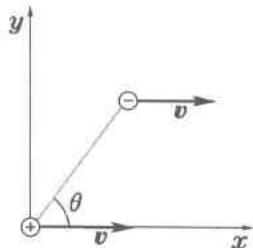
\includegraphics[width = 0.3\textwidth]{figures/习题3-24.jpg}
\end{center}

\vfill
\newpage

\textbf{3-25.} 一螺绕环横截面的半径为 $a$ ，中心环线的半径为 $R, R \gg a$ ，其上由表面绝缘的导线均匀地密绕两个线圈，一个 $N_{1}$ 匝，另一个 $N_{2}$ 匝，求两线圈的互感 $M$ .


\vfill

\textbf{3-26.} 一圆形线圈由 50 匝表面绝缘的细导线绕成，圆面积为 $S = 4.0\mathrm{cm}^2$ . 放在另一个半径 $R = 20\mathrm{cm}$ 的大圆形线圈中心，两者同轴，如本题图所示，大圆形线圈由100匝表面绝缘的导线绕成。

(1) 求这两线圈的互感 M;

(2) 当大圆形导线中的电流每秒减小50A时，求小线圈中的感应电动势.
\begin{center}
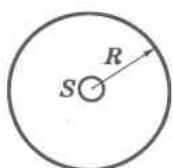
\includegraphics[width=0.2\linewidth]{figures/习题3-26.jpg}
\end{center}

\vfill
\newpage

\textbf{3-27.} 如本题图,一矩形线圈长 $a = 20\mathrm{cm}$ , 宽 $b = 10\mathrm{cm}$ , 由 100 匝表面绝缘的导线绕成, 放在一很长的直导线旁边并与之共面, 这长直导线是一个闭合回路的一部分, 其他部分离线圈都很远, 影响可略去不计。求图中 a 和 b 两种情况下, 线圈与长直导线之间的互感。

\begin{center}
    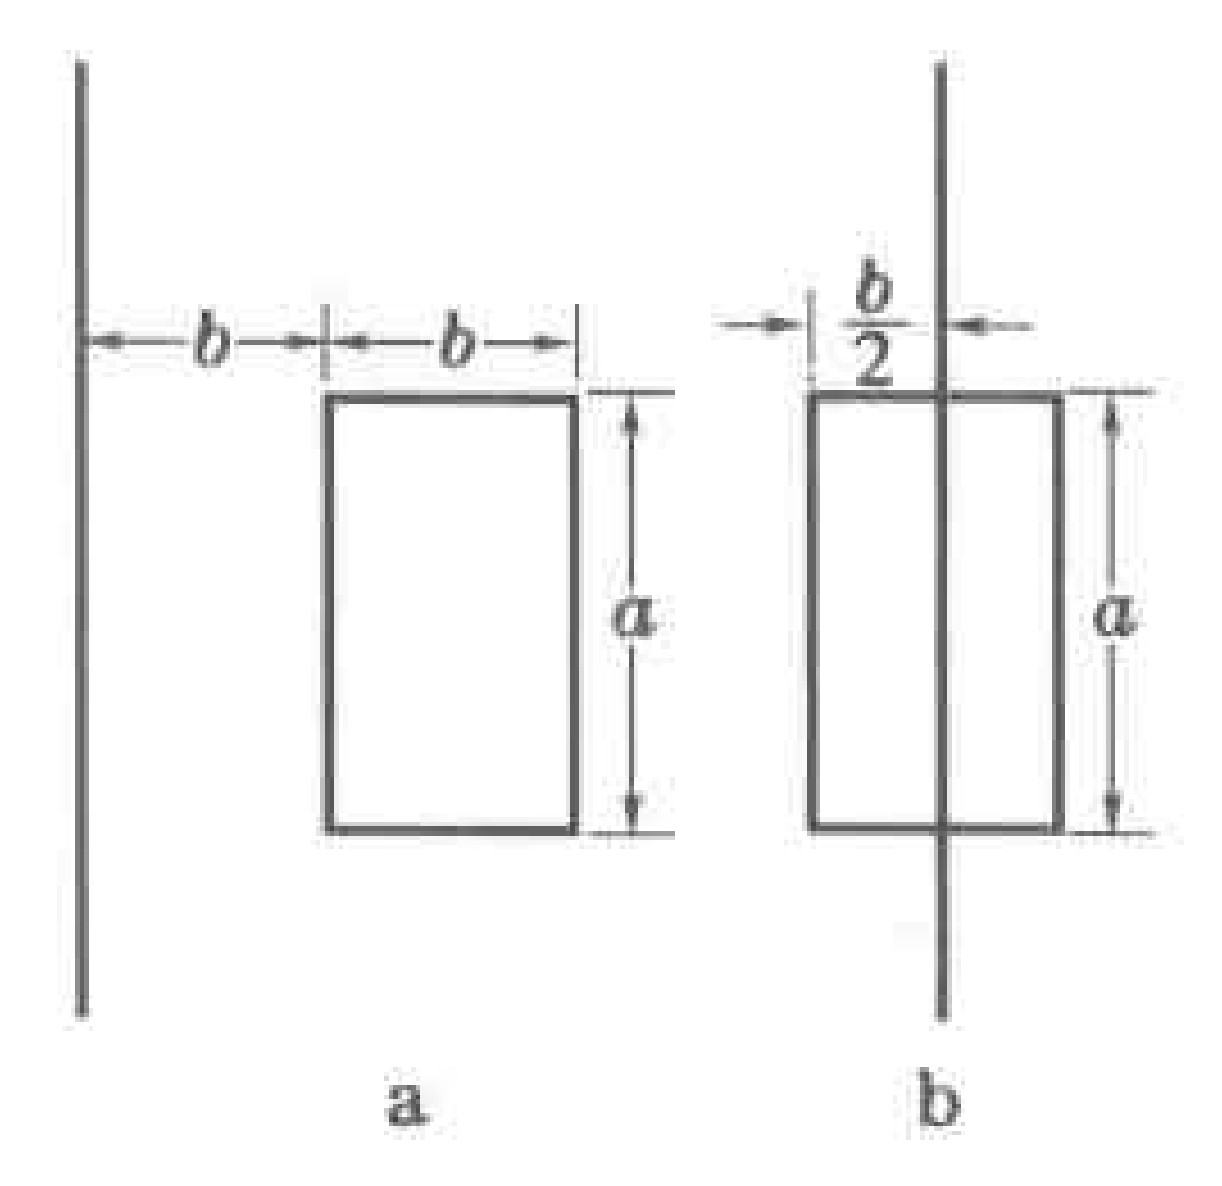
\includegraphics[width = 0.3\linewidth]{figures/习题3-27.jpg}
\end{center}

\vfill

\textbf{3-28.} 如本题图,两长螺线管同轴,半径分别为 $R_{1}$ 和 $R_{2}(R_{1} > R_{2})$ ,长度为 $l(l \gg R_{1}$ 和 $R_{2})$ ,匝数分别为 $N_{1}$ 和 $N_{2}$ . 求互感系数 $M_{12}$ 和 $M_{21}$ ,由此验证 $M_{12} = M_{21}$ .
\begin{center}
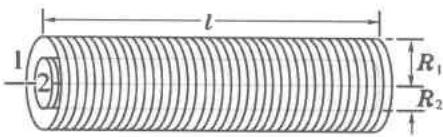
\includegraphics[width=0.4\linewidth]{figures/习题3-28.jpg}
\end{center}

\vfill
\newpage

\textbf{3-29.} 在长 $60\mathrm{cm}$ 、直径 $5.0\mathrm{cm}$ 的空心纸筒上绕多少匝导线，才能得到自感为 $6.0\times 10^{-3}\mathrm{H}$ 的线圈？

\vfill

\textbf{3-30.} 矩形截面螺绕环的尺寸如本题图, 总匝数为 N.

(1) 求它的自感系数；

(2) 当 N=1000 匝， $D_{1}=20\ cm$ ， $D_{2}=10\ cm$ ，h=1.0cm 时，自感为多少？

\begin{center}
    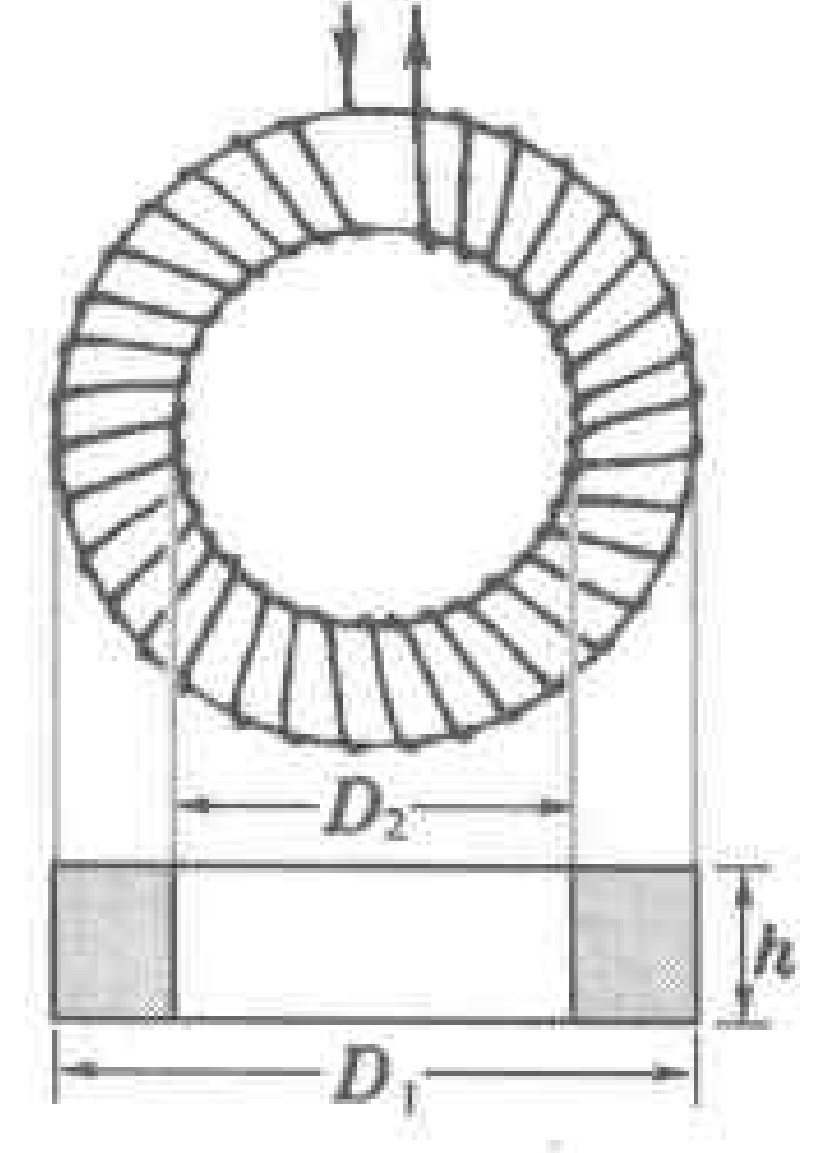
\includegraphics[width = 0.2\linewidth]{figures/习题3-30}
\end{center}


\vfill
\newpage

\textbf{3-31.} 两根平行导线，横截面的半径都是 $a$ ，中心相距为 $d$ ，载有大小相等而方向相反的电流。设 $d \gg a$ ，且两导线内部的磁通量都可略去不计。证明：这样一对导线长为 $l$ 的一段的自感为

\vfill

\textbf{3-32.} 在一纸筒上密绕有两个相同的线圈 $ab$ 和 $a'b'$ ，每个线圈的自感都是 $0.050\mathrm{H}$ ，如本题图所示。求：

(1) a 和 $a'$ 相接时, b 和 $b'$ 间的自感;

(2) $a'$ 和 b 相接时，a 和 $b'$ 间的自感。
\begin{center}
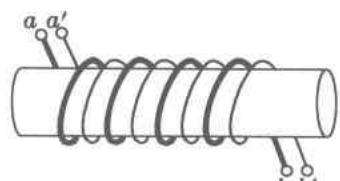
\includegraphics[width=0.3\linewidth]{figures/习题3-32.jpg}
\end{center}


\vfill
\newpage

\textbf{3-33.} 两线圈的自感分别为 $L_{1} = 5.0\mathrm{mH}$ , $L_{2} = 3.0\mathrm{mH}$ , 当它们顺接串联时, 总自感为 $L = 11.0\mathrm{mH}$ .

(1) 求它们之间的互感；

(2) 设这两线圈的形状和位置都不改变，只把它们反接串联，求它们反接后的总自感。

\vfill

\textbf{3-34.} 两线圈顺接后总自感为 $1.00\mathrm{H}$ , 在它们的形状和位置都不变的情况下, 反接后的总自感为 $0.40\mathrm{H}$ . 求它们之间的互感。

\vfill
\newpage

\textbf{3-35.} 两根足够长的平行导线间的距离为 $20\mathrm{cm}$ ，在导线中保持一大小为 $20\mathrm{A}$ 而方向相反的恒定电流。

(1) 求两导线间每单位长度的自感系数, 设导线的半径为 $1.0 \, mm$ ;

(2) 若将导线分开到相距 $40 \, cm$ ，求磁场对导线单位长度所作的功；

(3) 位移时，单位长度的磁能改变了多少？是增加还是减少？说明能量的来源。


\vfill
\newpage